\chapter{探测器、时钟与事件表}
\label{chap:e13}

\begin{chapteropening}
第 \ref{chap:e07} 章告诉我们，探测的本质是"吸收一个光子、吐出一次电脉冲"；第 \ref{chap:e08} 章又告诉我们，藏在事件流里的相关峰可以小到 \(10^{-6}\)，而且会被探测器有限的时间响应卷积展宽、稀释。可这两章都还停在"理想探测器"的层面。真实的望远镜没有理想探测器：光子撞上光阴极只有一定概率变成电子；每个电脉冲到来的时刻都带着几十皮秒到几纳秒的随机抖动；探测器每响一次就要"喘口气"，在这段死时间里对新光子视而不见；两台相距百米的望远镜，各自的时钟还得对齐到皮秒。本章要回答一个非常"硬件"的问题：一个光子，究竟经过哪些环节，才变成事件表里那一行\emph{带时间戳的记录}？我们会把量子效率、时间抖动、死时间与堆积、afterpulsing、时钟同步这几件事逐一拆开，把每一个公式从头推到尾，最后落到"事件表该存哪些字段"这张最实用的清单上。
\end{chapteropening}

\section{从光子到一行带时间戳的事件}
\label{sec:e13-from-photon-to-event}

先把上一阶段的结论接住。第 \ref{chap:e07} 章把"探测"讲成了一个概率事件：一个能量为 \(h\nu\) 的光子打到探测器上，有一定概率被吸收并触发一次可记录的电脉冲。第 \ref{chap:e08} 章把这些电脉冲排成一串带时间戳的"点击"，并教我们从中读出 \(g^{(2)}(\tau)\)。但那里的探测器是"透明"的——光子进去，事件出来，中间不损耗、不延迟、不饱和。真实器件恰恰相反：它在光子和事件之间设了好几道关卡，每一道关卡都会改写事件率、时间戳或峰形。本章就是要把这几道关卡一一打开。

关键的数据结构叫\textbf{事件表}（event list）。它和普通的光变曲线（light curve）有本质区别。光变曲线是"把一段曝光里的光子数累加到一个时间 bin 上"——一旦累加，谁在什么时刻来的、来自哪个望远镜、哪个波长、哪个偏振，全都糊成了一个数。事件表则相反，它\emph{逐个光子}保留信息：到达时刻、望远镜编号、探测器通道、波长通道、偏振通道、权重、质量标记。为什么值得这么"啰嗦"地存？因为二阶相关、脉冲星折叠、快速遮掩这些测量，信号恰恰藏在"哪两个光子几乎同时到达"这种联合信息里；只要过早地按时间 bin 累加，待测的相关峰就被抹掉了，事后再也补不回来。Iqueye 就是这么设计的：它把每个光子都打上时间标签保存，事后再离线选择从 24.41 ps 到分钟级的任意时间 bin；对 \(\zeta\) Ori 的一次观测就产生了约 \(2\times10^{10}\) 个光子事件、约 78 GB 数据 \citep{2009A&A...508..531N,2019CoSka..49...85Z}。可见事件表不是可有可无的辅助文件，而是真实望远镜的主要数据产品。

把一行原始事件写下来，它长这样：
\begin{equation}
  \mathcal{E}^{\rm raw}_q =
  \big(n_q,\ a_q,\ d_q,\ c_q,\ p_q,\ f_q,\ w_q\big),
  \qquad
  t^{\rm raw}_q=t_0+n_q\,\delta t+\epsilon_{\rm roll}.
  \label{eq:e13-raw-event}
\end{equation}
\begin{formulaexplain}
\(\mathcal E_q^{\rm raw}\) 是第 \(q\) 个原始事件；\(n_q\) 是时钟计数（tick），\(\delta t\) 是一个 tick 的时长，\(t_0\) 是记录段起点，\(\epsilon_{\rm roll}\) 处理计数器溢出。它把一次电子记录翻译成最早的事件时刻。
\end{formulaexplain}
逐个符号落实。下标 \(q\) 编号第 \(q\) 个事件。\(n_q\) 是电子计数器读到的整数 tick 数（无量纲）；\(\delta t\) 是一个 tick 对应的时间（单位秒），现代时间数字转换器（time-to-digital converter, TDC）的 \(\delta t\) 常在 \(10^{-11}\)--\(10^{-10}\,{\rm s}\) 量级，商用多通道 TCSPC 系统基本时间分辨率可到 80 ps，Iqueye 的量化步长是 24.41 ps \citep{2009A&A...508..531N,2020RScI...91a3108W}。\(t_0\) 是记录段的起始时刻（秒），\(\epsilon_{\rm roll}\) 处理计数器满量程后回绕（rollover）或分段。后面几个整数都是"标签"：\(a_q\) 是望远镜或站点编号，\(d_q\) 是探测器编号，\(c_q\) 是波长通道或滤光片编号，\(p_q\) 是偏振通道，\(f_q\) 是质量标记，\(w_q\) 是事件权重。溢出、丢包、饱和、云、指向异常、电子学异常都应该写进 \(f_q\)——否则日后相关函数里冒出一个诡异的峰，你将无从追溯它是天体还是故障。

\begin{figure}[tbp]
\centering
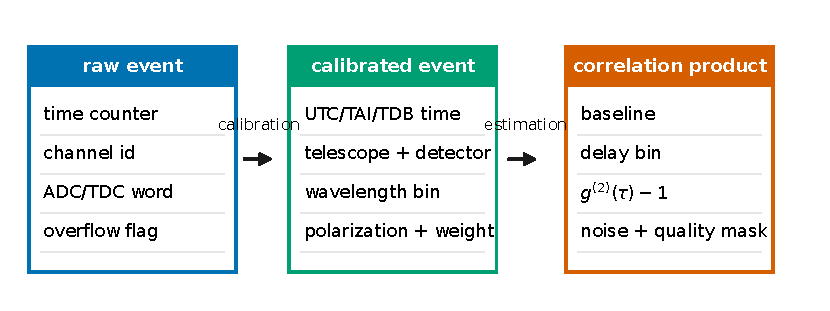
\includegraphics[width=0.96\linewidth]{figures/generated/chapter_06/ch06_event_table_schema.pdf}
\caption{事件数据从原始电子记录流向标定事件表，再流向相关函数产品。原始层保存计数器时间、通道编号和溢出标记；标定层把时间转换到统一时间尺度，并加入望远镜、波长、偏振和权重；相关产品层才记录基线、延迟 bin、相关幅度与噪声估计。若在第一层就只保存光变曲线，后面的时钟、波长和偏振选择都将无法重新执行。}
\label{fig:e13-event-table-schema}
\end{figure}

本章的路线也就清楚了：先看光子怎样以概率 \(\eta\) 变成电子事件（\ref{sec:e13-detectors} 节），再看每个事件时刻带着多大抖动、如何把相关峰卷宽（\ref{sec:e13-jitter} 节），接着看探测器"喘气"造成的死时间与堆积如何让记录率饱和（\ref{sec:e13-deadtime} 节）、afterpulsing 如何伪造短延迟相关（\ref{sec:e13-afterpulse} 节），然后把两台望远镜的时钟对齐到皮秒（\ref{sec:e13-clock} 节），最后落到事件表字段清单（\ref{sec:e13-schema} 节）和谱分辨与相干时间的权衡（\ref{sec:e13-spectral} 节）。

\section{探测器：量子效率把光子变成电子事件}
\label{sec:e13-detectors}

探测器的第一项、也是最基本的作用，是决定"有多少入射光子真的变成了电子事件"。这一步的核心参数叫\textbf{量子效率}（quantum efficiency）\(\eta\)：一个到达感光面的光子，被吸收并触发一次可计数脉冲的概率。它无量纲，取值在 0 和 1 之间，而且强烈依赖波长。把整条光路的效率乘起来，一个通道的平均探测率是
\begin{equation}
  R_{\rm det}
  =
  A_{\rm eff}
  \int_{\lambda_1}^{\lambda_2}
  F_\lambda(\lambda)\,
  T_{\rm opt}(\lambda)\,
  \eta(\lambda)\,
  d\lambda
  \;+\;R_{\rm sky}+R_{\rm dark}.
  \label{eq:e13-detected-rate}
\end{equation}
\begin{formulaexplain}
\(R_{\rm det}\) 是探测计数率；\(A_{\rm eff}\) 是有效集光面积；\(F_\lambda\)、\(T_{\rm opt}\)、\(\eta\) 分别是源光子谱通量、光路透过率和量子效率；\(R_{\rm sky},R_{\rm dark}\) 是天光背景与暗计数。它是一份"事件率预算"。
\end{formulaexplain}
逐项交代单位与量级。\(A_{\rm eff}\) 是有效集光面积（\({\rm m}^2\)），对大气 Cherenkov 望远镜可达几十到上百 \({\rm m}^2\)。\(F_\lambda\) 是源的光子谱通量密度（\({\rm photons\,s^{-1}\,m^{-2}\,nm^{-1}}\)）。\(T_{\rm opt}\) 是镜面、滤光片、光纤、准直器、窗口的总透过率（无量纲，通常远小于 1）。\(\eta(\lambda)\) 是量子效率。\(R_{\rm sky}\) 是天光和杂散光的计数率，\(R_{\rm dark}\) 是探测器在完全无光时也会自发产生的暗计数率（两者单位都是 \({\rm s}^{-1}\)）。式子的结构很直白：源贡献是"面积 × 谱通量 × 透过率 × 效率"在带宽内的积分，再加上两项与源无关的背景。强度干涉的信噪比，最终就由"被背景稀释后的恒星光子率与强度起伏"共同决定；MAGIC-SII 直接用 PMT 直流电流估计光子通量、用背景像素修正夜天光，VERITAS-SII 用 off-source 测量估计背景再把相关幅度按恒星光占比修正 \citep{2020NatAs...4.1164A,2024MNRAS.529.4387A}。

不同任务要用不同探测器，它们在"效率、时间分辨、面积、暗计数"之间各有取舍。把常见的几类摆在一起看：

\begin{itemize}
  \item \textbf{光电倍增管（PMT，photomultiplier tube）}：光子打在光阴极上打出光电子，经过一串打拿极（dynode）逐级倍增，增益可达 \(10^6\) 量级。它面积大、增益高、脉冲窄（ns 级），和 Cherenkov 望远镜的高速电子链天然匹配；蓝光量子效率常在 \(20\%\)--\(40\%\)，VERITAS-SII 在 416 nm 使用的 PMT 量子效率约 \(30\%\) \citep{2020NatAs...4.1164A,2024MNRAS.529.4387A}。它是当代地面强度干涉的主力探测器。
  \item \textbf{雪崩光电二极管（APD，avalanche photodiode）}：半导体器件，靠反向偏压下的雪崩倍增放大信号。工作在偏压低于击穿电压的\emph{线性模式}时，输出正比于入射光强，增益适中、噪声较低，适合中等到较强光通量，但通常不做单光子计数。
  \item \textbf{单光子雪崩二极管（SPAD，single-photon avalanche diode）}：把 APD 偏置到\emph{击穿电压以上}（盖革模式，Geiger mode），一个光电子就能触发一次自持雪崩，产生一个"有/无"的数字脉冲。可见光量子效率可达 \(50\%\)--\(60\%\)，单光子时间分辨率约 30--50 ps，暗计数常见 10--100 \({\rm s}^{-1}\)；代价是感光面积小、死时间较长，而且雪崩后会有 afterpulsing 污染短延迟相关（下文详述）\citep{1996ApOpt..35.1956C,2009JMOp...56..261B,2009A&A...508..531N,2015SPIE.9504E..0CZ}。
  \item \textbf{硅光电倍增管（SiPM，silicon photomultiplier）}：把成百上千个微小 SPAD 单元（microcell）并联成一块面阵，每个单元只报"有/无"，把它们的输出相加就得到近似正比于光子数的信号。它兼顾了单光子灵敏度与较大的有效面积，供电低、不怕强光损伤，已进入新一代 Cherenkov 相机；代价是单元间存在光学串扰（optical crosstalk），暗计数率也比单个 SPAD 高。
  \item \textbf{超导纳米线单光子探测器（SNSPD，superconducting nanowire single-photon detector）}：把一根偏置到临界电流附近的超导纳米线冷却到几开尔文，一个光子被吸收就足以破坏局部超导态、产生一个可记录的电压脉冲。它同时做到高量子效率（可达 \(90\%\) 以上）、极低暗计数（可低至 \({\rm s}^{-1}\) 量级以下）和皮秒级时间抖动，是当前计时与暗计数综合性能最强的单光子探测器；代价是需要低温制冷系统、感光面积小。
  \item \textbf{能量分辨型探测器（如 MKID，microwave kinetic inductance detector，微波动电感探测器）}：这类超导器件在吸收一个光子后，其超导动电感随入射光子能量而变，因而能\emph{直接读出每个光子的波长}，天生自带光谱通道。代价是时间分辨率通常只到微秒量级、死时间长，且同样需要低温系统——它用时间分辨换取了能量（波长）分辨。
\end{itemize}

\begin{figure}[tbp]
\centering
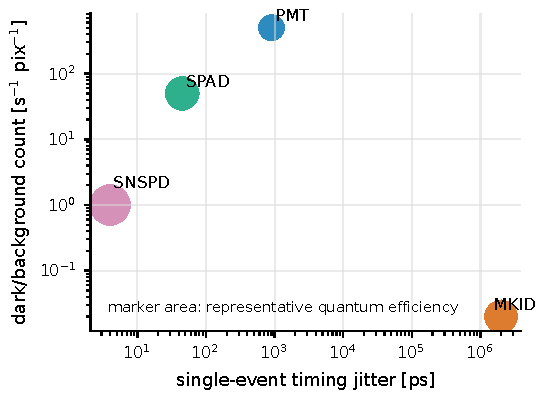
\includegraphics[width=0.72\linewidth]{figures/generated/chapter_06/ch06_detector_trade_space.pdf}
\caption{几类单光子探测技术的典型工作区域。横轴是单事件时间抖动，纵轴是每像素暗计数或背景计数的代表值，点面积表示代表性量子效率。PMT 适合大口径、高通量和 ns 级强度干涉；SPAD 给出几十皮秒计时但受面积与死时间限制；超导器件在低暗计数与皮秒计时上最强，但需要低温系统；能量分辨型探测器则牺牲时间分辨换取每个光子的波长信息。}
\label{fig:e13-detector-trade-space}
\end{figure}

一句话把这一节收住：\(\eta\) 决定\emph{有多少}光子变成事件，进而决定信噪比里的"信号"；而"事件何时到、探测器多久能再响一次"这些时间性质，决定了事件表里的相关结构还忠不忠实于入射光场——这正是接下来三节要拆的东西。

\section{时间抖动：相关峰为什么会被展宽}
\label{sec:e13-jitter}

第 \ref{chap:e08} 章已经预告：探测器有限的时间响应会把窄相关峰卷积展宽、峰高稀释。现在我们把这件事讲透。问题的根源是\textbf{时间抖动}（timing jitter）：即便同一个光子在同一时刻到达，探测器输出脉冲被判定为"事件"的那个时刻，每次都略有不同，是一个随机量。对 SPAD 约几十皮秒，对 PMT 加电子链可到 ns 级。把这种随机延迟写成一个响应函数 \(h(t)\)（归一化的概率分布，描述"真实到达时刻 0 对应的记录时刻分布"），那么观测到的事件时间就是真实时间与 \(h\) 的卷积。

对二阶相关，两个通道各有响应 \(h_1(t)\)、\(h_2(t)\)，观测到的相关超额是天体真实相关与合成响应的卷积：
\begin{equation}
  C^{\rm obs}_{12}(\tau)
  =
  \int C^{\rm sky}_{12}(\tau')\,
  h_{12}(\tau-\tau')\,d\tau',
  \qquad
  h_{12}=h_1*h_2.
  \label{eq:e13-response-convolution}
\end{equation}
\begin{formulaexplain}
\(C^{\rm sky}_{12}\) 是天体真实相关，\(C^{\rm obs}_{12}\) 是观测结果；\(h_1,h_2\) 是两通道时间响应，\(h_{12}\) 是它们的卷积。仪器把窄相关峰"抹宽"。
\end{formulaexplain}
这里 \(C_{12}=g^{(2)}_{12}-1\)（无量纲），\(\tau,\tau'\) 单位是秒，\(*\) 是卷积。物理图像很直白：真实相关峰无限窄也没用，因为你根本不知道每个光子的\emph{准确}到达时刻，只知道它落在一个宽约 \(\sigma\) 的模糊窗口里；两路模糊叠加，观测峰就被展宽到 \(h_{12}\) 的宽度。

要把"展宽多少"算清楚，用一个非常好用的近似：把每个响应都当作高斯。这里要点名一个标准结果——\emph{两个高斯函数的卷积仍是高斯，且方差相加}。设 \(h_1\) 是宽度（方差）\(\sigma_1^2\) 的高斯、\(h_2\) 是 \(\sigma_2^2\) 的高斯，则
\[
  h_{12}=h_1*h_2 \;\Longrightarrow\; \sigma_{12}^2=\sigma_1^2+\sigma_2^2 .
\]
把源自身的宽度、光路展宽、时钟残差也一并算进来，各项若彼此独立，方差就直接相加（这叫"按方差相加"，是独立高斯展宽叠加的普遍规则）：
\begin{equation}
  \sigma_{\rm obs}^2
  \simeq
  \sigma_{\rm sky}^2+\sigma_1^2+\sigma_2^2+\sigma_{\rm opt}^2+\sigma_{\rm clk}^2 .
  \label{eq:e13-jitter-budget}
\end{equation}
\begin{formulaexplain}
\(\sigma_{\rm obs}\) 是观测峰宽；\(\sigma_{\rm sky}\) 是源自身宽度，\(\sigma_1,\sigma_2\) 是两探测器抖动，\(\sigma_{\rm opt}\) 是光路展宽，\(\sigma_{\rm clk}\) 是时钟残差。独立高斯展宽按方差相加。
\end{formulaexplain}
每一项都是 rms 时间宽度（秒）。\(\sigma_{\rm sky}\) 是光源的相干时间或脉冲宽度，\(\sigma_1,\sigma_2\) 是探测器与电子通道的抖动，\(\sigma_{\rm opt}\) 是镜面等时性误差（比如 Davies--Cotton 镜面不同格子的光程差），\(\sigma_{\rm clk}\) 是两站时钟对齐后的残差。这里有个重要的"数量级落地"：可见光宽带的相干时间 \(\tau_c\) 短到皮秒（第 \ref{chap:e02} 章），比 ns 级的 \(\sigma_1,\sigma_2\) 小了三个数量级，于是式 \eqref{eq:e13-jitter-budget} 里 \(\sigma_{\rm sky}\) 项几乎可以忽略——\emph{观测峰宽几乎完全由仪器决定}。VERITAS 的镜面加 PMT 脉冲宽度使强度相关峰可用 \(\sigma_\tau\simeq4\,{\rm ns}\) 的高斯描述，MAGIC-SII 的相关峰高斯宽度约 \(2.2\,{\rm ns}\) \citep{2020NatAs...4.1164A,2024MNRAS.529.4387A}。

这带来一个关键后果：\emph{峰宽变了，峰高也跟着变}。因为相关峰下的"面积"（真实相关的总强度）在卷积中近似守恒，把它摊到更宽的峰上，峰高就按展宽因子被稀释。若真实峰宽 \(\sigma_{\rm sky}\ll\sigma_{\rm obs}\)，观测峰高相对真实峰高大约被压低了一个 \(\sigma_{\rm sky}/\sigma_{\rm obs}\) 的因子。这就是第 \ref{chap:e08} 章说"相关峰会被时间响应稀释"的定量来源，也解释了为什么强度干涉要拼命追求高电子带宽和稳定的响应函数——响应越窄，峰高稀释越少，越容易把 \(10^{-6}\) 量级的峰从噪声里挑出来。

\begin{figure}[tbp]
\centering
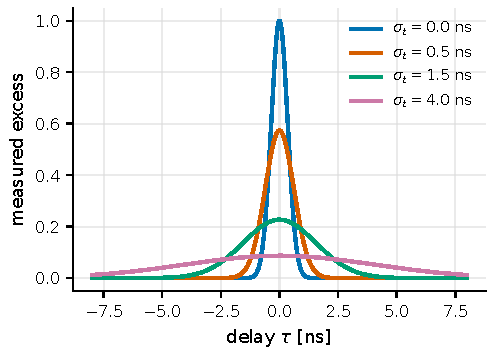
\includegraphics[width=0.72\linewidth]{figures/generated/chapter_06/ch06_detector_timing_response.pdf}
\caption{有限时间响应把窄相关峰展宽并降低峰高。曲线保持峰面积近似不变，只改变 rms 抖动 \(\sigma_t\)。当真实相干时间远短于 ns 级电子响应时，峰宽主要由仪器决定，峰高按展宽因子被稀释；这正是强度干涉需要高电子带宽和稳定响应函数的原因。}
\label{fig:e13-detector-timing-response}
\end{figure}

\section{死时间与堆积：记录率为什么会饱和}
\label{sec:e13-deadtime}

抖动改变的是每个事件的\emph{时刻}；死时间改变的是\emph{有多少事件}能被记下来。\textbf{死时间}（dead time）\(\tau_d\) 是探测器响一次之后"喘气"的一段时间，在此期间它对新光子视而不见。当光子来得又快又密，死时间就会吃掉大量事件，让记录率 \(r_{\rm rec}\) 明显低于真实入射率 \(r\)——这叫\textbf{堆积}（pile-up）造成的计数损失。这里有一个微妙但重要的分岔：死时间到底会不会被"死时间里到来的光子"再次刷新？两种回答给出两种模型，务必分清。

\paragraph{非麻痹型：死时间不被刷新}

先看\textbf{非麻痹型}（non-paralyzable）。它假设：探测器记下一个事件后死 \(\tau_d\)，这段时间里来的光子一律丢弃，\emph{但不会延长}死时间；\(\tau_d\) 一到，探测器立刻复活等下一个。推导用一个"活时间账本"的办法，零跳步地做出来。

设总观测时长为 \(T\)，真实入射率为 \(r\)（\({\rm s}^{-1}\)），记录到的事件总数为 \(M\)。每记录一个事件就死 \(\tau_d\)，所以总死时间是 \(M\tau_d\)，于是探测器真正"活着、能响应"的时间是
\[
  T_{\rm live}=T-M\tau_d .
\]
非麻痹型的关键是：只有在活时间里到来的光子才会被记录，而在活时间里，光子以真实率 \(r\) 泊松地到来，所以
\[
  M=r\,T_{\rm live}=r\,(T-M\tau_d).
\]
把含 \(M\) 的项归拢：
\[
  M=rT-rM\tau_d \;\Longrightarrow\; M+rM\tau_d=rT \;\Longrightarrow\; M(1+r\tau_d)=rT .
\]
两边除以 \(T\)，记 \(r_{\rm rec}=M/T\)，就得到记录率：
\begin{equation}
  r_{\rm rec}=\frac{r}{1+r\tau_d}.
  \label{eq:e13-nonparalyzable}
\end{equation}
\begin{formulaexplain}
\(r\) 是真实入射率，\(r_{\rm rec}\) 是记录率，\(\tau_d\) 是死时间。非麻痹型里死时间内的光子被丢弃、但不延长恢复窗口，所以 \(r_{\rm rec}\) 随 \(r\) 单调上升并饱和到 \(1/\tau_d\)。
\end{formulaexplain}
读一下这条式子的极限。低通量 \(r\tau_d\ll1\) 时分母趋近 1，\(r_{\rm rec}\approx r(1-r\tau_d)\)，损失很小；高通量 \(r\tau_d\gg1\) 时 \(r_{\rm rec}\to 1/\tau_d\)——记录率\emph{饱和}到一个上限，探测器每 \(\tau_d\) 顶多报一个事件，再多的光子也挤不进来，但绝不会倒退。

\paragraph{麻痹型：每个光子都刷新死时间}

再看\textbf{麻痹型}（paralyzable）。它假设：死时间内到来的每一个新光子，虽然\emph{不被记录}，却会\emph{重新触发}一段 \(\tau_d\) 的死时间。于是只有当一个光子到来时、它前面已经\emph{空了至少 \(\tau_d\)}没有任何光子，这个光子才会被记录。

推导要用泊松过程的一条标准结果：对速率为 \(r\) 的泊松过程，相邻两个光子之间的时间间隔服从指数分布，\emph{间隔超过 \(\tau_d\) 的概率是 \(e^{-r\tau_d}\)}。（这就是"在长度 \(\tau_d\) 的窗口里一个光子都没有"的概率，等于泊松分布取 0 个：\(P(0)=e^{-r\tau_d}\)。）一个到来的光子能被记录，当且仅当它之前的那段空窗大于 \(\tau_d\)。所有光子以率 \(r\) 到来，其中"前置空窗 \(>\tau_d\)"的那一部分才算数，所以记录率是
\[
  r_{\rm rec}=r\times P(\text{前置间隔}>\tau_d)=r\,e^{-r\tau_d}.
\]
写成编号式子：
\begin{equation}
  r_{\rm rec}=r\,e^{-r\tau_d}.
  \label{eq:e13-paralyzable}
\end{equation}
\begin{formulaexplain}
同样是死时间模型，但每个到来的光子都会刷新恢复窗口。因此 \(r_{\rm rec}\) 在 \(r\tau_d=1\) 处达到最大，之后随 \(r\) 增大反而\emph{下降}——高通量下探测器几乎一直被刷新、报不出事件。
\end{formulaexplain}
读极限：低通量 \(r\tau_d\ll1\) 时 \(e^{-r\tau_d}\approx1-r\tau_d\)，\(r_{\rm rec}\approx r(1-r\tau_d)\)——和非麻痹型在低通量下\emph{完全一致}，这也是为什么弱光下两种模型很难区分。但高通量截然不同：把 \(r_{\rm rec}=re^{-r\tau_d}\) 对 \(r\) 求导，\(\frac{d r_{\rm rec}}{dr}=e^{-r\tau_d}(1-r\tau_d)\)，在 \(r\tau_d=1\)（即 \(r=1/\tau_d\)）处为零，是个极大值，峰值 \(r_{\rm rec}^{\max}=1/(e\tau_d)\approx0.368/\tau_d\)；再往上，光子密到彼此不断刷新死时间，记录率\emph{掉头向下}，极端时探测器几乎瘫痪（paralyzed，模型因此得名）。

\paragraph{对比与数量级}

把两条式子并排读，物理差别一句话：非麻痹型高通量下\emph{饱和}到 \(1/\tau_d\)，麻痹型高通量下\emph{回落}。这个差别在实验上要命——如果你误把麻痹型当非麻痹型，在高计数率下会严重高估真实率。所以真实仪器必须\emph{单独测出}自己属于哪一类、\(\tau_d\) 是多少，办法是用可调强度的稳定光源画出 \(r_{\rm rec}\) 对 \(r\) 的曲线，看它到底是饱和还是回落。

代进数字体会量级。取一个高速单光子通道的典型死时间 \(\tau_d=20\,{\rm ns}=2\times10^{-8}\,{\rm s}\)：
\[
  r=10^7\,{\rm s^{-1}}:\quad r\tau_d=0.2,\quad
  r_{\rm rec}^{\rm non}=\frac{10^7}{1.2}\approx8.3\times10^6\,{\rm s^{-1}},
\]
即已经损失约 \(17\%\)；同一入射率下麻痹型 \(r_{\rm rec}=10^7e^{-0.2}\approx8.2\times10^6\,{\rm s^{-1}}\)，两者几乎一样。再升到 \(r=10^8\,{\rm s^{-1}}\)（\(r\tau_d=2\)）：非麻痹型 \(r_{\rm rec}=10^8/3\approx3.3\times10^7\,{\rm s^{-1}}\)，还在爬；麻痹型 \(r_{\rm rec}=10^8e^{-2}\approx1.35\times10^7\,{\rm s^{-1}}\)，\emph{已经越过峰值往下掉了}（峰值出现在 \(r=1/\tau_d=5\times10^7\,{\rm s^{-1}}\)，此时 \(r_{\rm rec}^{\max}\approx1.84\times10^7\,{\rm s^{-1}}\)）。SPAD 常见死时间几十 ns 到几百 ns，能量分辨型探测器可到 \(100\,\mu{\rm s}\) 量级，现代 TCSPC 电子学本身可把通道死时间压到 650 ps，但探测器脉冲宽度和前端电子仍会限制真实高通量能力 \citep{2009A&A...508..531N,2013PASP..125.1348M,2020RScI...91a3108W}。

\begin{figure}[tbp]
\centering
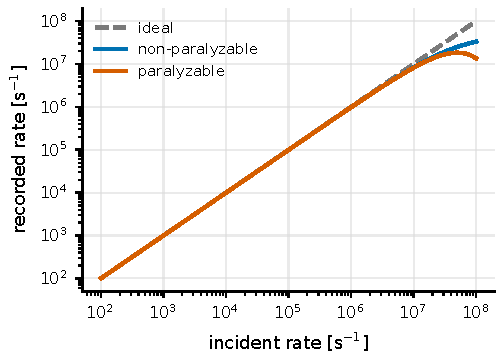
\includegraphics[width=0.72\linewidth]{figures/generated/chapter_06/ch06_deadtime_saturation.pdf}
\caption{入射计数率升高时，死时间使记录计数率偏离理想直线。非麻痹型趋向饱和值 \(1/\tau_d\)，麻痹型在极高通量下反而下降。图中取 \(\tau_d=20\,{\rm ns}\)，代表高速单光子通道的数量级；真实仪器需要用可调强度光源单独测量 \(\tau_d\) 与模型类型。}
\label{fig:e13-deadtime-saturation}
\end{figure}

死时间还提示了强度干涉常用的一招：把光\textbf{分束到两个独立探测器}做互相关（HBT 的做法，见第 \ref{chap:e10} 章）。因为死时间是\emph{每个探测器各自}的，两个探测器不会因为对方在死时间而漏掉零延迟附近的符合；这样既提高了可承受的总计数率，又顺带压掉了下一节要讲的同通道 afterpulsing \citep{1957RSPSA.242..300B,1996ApOpt..35.1956C,2020RScI...91a3108W}。

\section{Afterpulsing：探测器自造的短延迟假相关}
\label{sec:e13-afterpulse}

死时间让事件\emph{变少}，afterpulsing 却让事件\emph{无中生有}。在雪崩型器件（SPAD、SiPM）里，一次雪崩会有部分载流子被材料缺陷"抓住"（陷阱，trap），过一会儿又被释放，重新触发一次和天体光子毫无关系的二次脉冲——这就是\textbf{余脉冲}（afterpulse）。它危险的地方在于：这些假脉冲总是紧跟在真实脉冲后面几 ns 到几 \(\mu\)s，恰好落在我们最关心的\emph{短延迟}区间，会在自相关里伪造出一个假峰，被误读成"光子结伴到达"。

把它写成率的形式。设每个真实事件产生一个 afterpulse 的概率是 \(\epsilon_{\rm ap}\)，这些余脉冲相对主脉冲的延迟服从归一化分布 \(k_{\rm ap}(\tau)\)，那么额外的事件率是
\begin{equation}
  R_{\rm ap}(\tau)=\epsilon_{\rm ap}\,R_{\rm det}\,k_{\rm ap}(\tau),
  \qquad
  \int_0^\infty k_{\rm ap}(\tau)\,d\tau=1.
  \label{eq:e13-afterpulse}
\end{equation}
\begin{formulaexplain}
\(R_{\rm ap}\) 是余脉冲贡献；\(\epsilon_{\rm ap}\) 是每个真实事件产生余脉冲的概率；\(R_{\rm det}\) 是真实探测率；\(k_{\rm ap}\) 是归一化延迟核。它描述探测器\emph{自己制造}的短延迟假相关。
\end{formulaexplain}
逐项落实。\(\epsilon_{\rm ap}\) 无量纲，随器件与门控方式在 \(10^{-4}\)--\(10^{-2}\) 之间；\(R_{\rm det}\) 是式 \eqref{eq:e13-detected-rate} 给出的探测率（\({\rm s}^{-1}\)）；\(k_{\rm ap}(\tau)\) 单位是 \({\rm s}^{-1}\)（因为对 \(\tau\) 积分归一），它的特征时间从 ns 到 \(\mu\)s 不等。式子结构是"真实事件率 × 单次余脉冲概率 × 延迟分布"，非常好记。

怎么和真信号区分开？两个办法。第一，\emph{对同一探测器}做自相关，你会看到 afterpulse 峰赫然出现在短延迟处；第二，\emph{对两个独立探测器}做互相关，因为 A、B 两个探测器的陷阱释放彼此独立、不同步，余脉冲不会在互相关里制造符合，于是被大幅压制。这又一次说明了 HBT 分束互相关的双重好处：既解决死时间，又躲开 afterpulsing——同一份光，分给两只"互不知情"的探测器，谁也没法用自己的毛病去污染彼此的符合计数 \citep{1957RSPSA.242..300B,1996ApOpt..35.1956C,2020RScI...91a3108W}。

\section{时钟与同步：把两台望远镜放到同一根时间轴上}
\label{sec:e13-clock}

到这里，一台望远镜内部的事件表已经建立好了。可强度干涉、甚长基线计时至少需要\emph{两台}望远镜，它们各自的事件表只有放到\emph{共同的时间轴}上才能相关。这就要求两站的时钟对齐得足够准。多准才够？这里有一条贯穿全书的换算，把"时间精度"翻译成"光走的距离"：
\begin{equation}
  \Delta\ell = c\,\Delta t .
  \label{eq:e13-lightpath}
\end{equation}
\begin{formulaexplain}
\(\Delta t\) 是两站时钟对齐的残差，\(c\) 是光速，\(\Delta\ell\) 是这段时间里光走过的距离。它把"同步到多少皮秒"直接换算成"等价于多少厘米光程"。
\end{formulaexplain}
这条式子其实就是第 \ref{chap:e01} 章用到的"时间-光程"对应，只是这次用在时钟上。代数字（CGS，\(c=3\times10^{10}\,{\rm cm\,s^{-1}}\)）：\(\Delta t=1\,{\rm ns}=10^{-9}\,{\rm s}\) 对应 \(\Delta\ell=30\,{\rm cm}\)；\(\Delta t=100\,{\rm ps}\) 对应 \(3\,{\rm cm}\)；\(\Delta t=1\,{\rm ps}\) 对应 \(0.3\,{\rm mm}\)。所以"把两站同步到皮秒-纳秒"，物理上就等价于"把两条光路的长度对齐到毫米-厘米"——一个非常直观的尺度。反过来，只要你把时钟对齐到几十皮秒，几厘米以内的光程差就被时钟吸收掉了。

实现这种同步有两条主流路线。一是\textbf{GPS 授时}：卫星广播的秒脉冲（PPS，pulse per second）给每站一个共同的绝对时刻，配上本地铷钟保持短期稳定；AquEYE/Iqueye 用铷钟加 GPS PPS，把\emph{相对}时间精度做到约 100 ps rms、\emph{绝对} UTC 精度控制在 \(0.5\,{\rm ns}\) 以内 \citep{2009A&A...508..531N,2015SPIE.9504E..0CZ}。二是 \textbf{White Rabbit}：一种基于以太网加精密相位测量的光纤同步协议，把一个主时钟通过光纤分发到各站并实时补偿光纤长度，5 km 光纤链路测试得到约 39 ps 的同步贡献——按式 \eqref{eq:e13-lightpath} 换算，只等价于约 1.2 cm 的光程残差 \citep{2013NIMPA.725..187J,2020RScI...91a3108W}。

有了共同时钟，还要扣掉一个更大的、\emph{随时间变化}的项——几何延迟。同一束星光到达两站的时刻本就不同，因为两站到源的光程不等。对一对站点 \(a,b\)：
\begin{equation}
  \Delta t_{\rm geo}(t)
  =
  \frac{\mathbf{B}_{ab}(t)\cdot\hat{\mathbf{s}}}{c},
  \qquad
  \mathbf{B}_{ab}=\mathbf{r}_b-\mathbf{r}_a .
  \label{eq:e13-geometric-delay}
\end{equation}
\begin{formulaexplain}
\(\Delta t_{\rm geo}\) 是两站几何延迟；\(\mathbf B_{ab}\) 是基线向量（由两站位置之差给出），\(\hat{\mathbf s}\) 是源方向单位矢量，\(c\) 是光速。它把空间基线\emph{投影}成两路事件表需要相互平移的时间量。
\end{formulaexplain}
\(\mathbf B_{ab}\) 单位是 m，\(\hat{\mathbf s}\) 无量纲，点积 \(\mathbf B_{ab}\cdot\hat{\mathbf s}\) 是基线在源方向上的投影长度，除以 \(c\) 就是时间。代数字：100 m 基线最高约 \(\Delta t_{\rm geo}=100/(3\times10^8)\approx333\,{\rm ns}\)（此最大值出现在源方向与基线平行、即近地平时；反之源在天顶、基线近水平时投影 \(\mathbf B_{ab}\cdot\hat{\mathbf s}\approx0\)，几何延迟接近零），1 km 基线约 \(3.3\,\mu{\rm s}\)——远大于皮秒级的探测器抖动，可见几何延迟是相关里\emph{最大}的时间项，必须先扣掉才能对齐零延迟。更麻烦的是它\emph{随时间漂移}：地球自转让投影基线不断改变，一个 100 m 基线在天顶（中天）附近漂移最快，延迟变化速度约 \(\Omega_\oplus B/c\sim2.4\times10^{-11}\,{\rm s\,s^{-1}}\)，其中 \(\Omega_\oplus\approx7.3\times10^{-5}\,{\rm rad\,s^{-1}}\) 是地球自转角速度；这意味着每 1 秒就漂约 \(24\,{\rm ps}\)（17 分钟累计约 \(25\,{\rm ns}\)）——对皮秒级峰形，这不能用一个常数延迟一劳永逸地吸收。VERITAS-SII 对每个相关帧移动时间 lag 校正几何光程，MAGIC-SII 在 Pearson 相关后施加可变时间延迟校正 \citep{2020NatAs...4.1164A,2024MNRAS.529.4387A}。

若还要把光子折叠到脉冲星相位、或与其他波段的到达时刻比较，站点时间还得进一步转换到\emph{太阳系质心}（Solar System barycenter, SSB），加上一串标准改正项——本地时钟到坐标时的转换、Roemer 光行时（地球绕日轨道给出最高约 \(\pm500\,{\rm s}\)）、Einstein 引力/运动钟速改正、Shapiro 引力延迟、大气延迟。这些改正 Tempo2 已做到 ns 级，barycorrpy 和 Astropy 提供 Python 工作流接口 \citep{2006MNRAS.369..655H,2006MNRAS.372.1549E,2018RNAAS...2....4K,2013A&A...558A..33A,2018AJ....156..123A}。这些属于绝对计时的进阶内容，本章只需记住：同夜强度相关看\emph{相对}延迟，脉冲相位和多信使比较才需要\emph{绝对}的质心时间。

\begin{figure}[tbp]
\centering
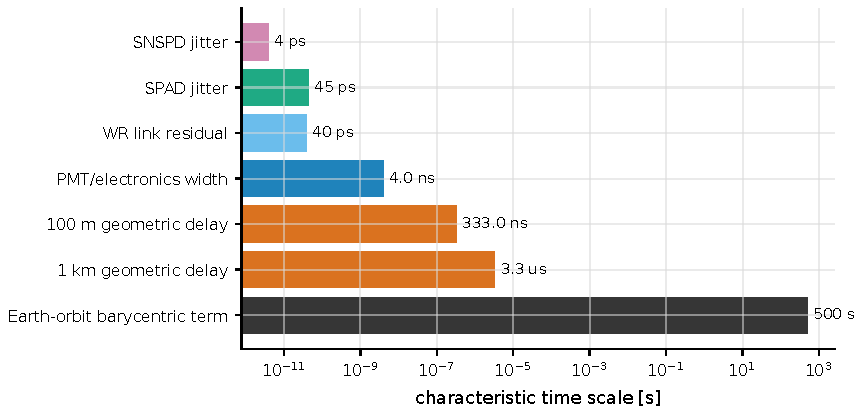
\includegraphics[width=0.84\linewidth]{figures/generated/chapter_06/ch06_time_budget.pdf}
\caption{同一份事件表会同时遇到皮秒、纳秒、微秒和百秒量级的时间项。探测器抖动与 White Rabbit 残差决定相关峰能否保持窄形；电子与镜面响应决定 ns 级强度干涉峰宽；几何延迟由基线长度与源方向决定，并随地球自转漂移；太阳系质心改正虽不是同夜峰宽项，却是脉冲相位、跨夜合并与多信使比较的绝对时间基础。}
\label{fig:e13-time-budget}
\end{figure}

把这些延迟一并写进标定事件表，原始计数器时间就变成了可跨站比较的物理时间：
\begin{equation}
  t^{\rm cal}_q =
  t^{\rm raw}_q
  +\Delta_{\rm clk}(t_q)
  +\Delta_{\rm elec}(a_q,d_q)
  +\Delta_{\rm det}(\lambda_q,d_q)
  -\frac{\mathbf{r}_{a_q}(t_q)\cdot\hat{\mathbf{s}}}{c}.
  \label{eq:e13-calibrated-time}
\end{equation}
\begin{formulaexplain}
\(t_q^{\rm cal}\) 是校正后事件时间；\(\Delta_{\rm clk},\Delta_{\rm elec},\Delta_{\rm det}\) 分别改正时钟、电子链路、探测器延迟；最后一项扣除几何光行时。它把不同站点放到共同时间轴。
\end{formulaexplain}
\(\Delta_{\rm clk}\) 是本站时钟相对统一时间尺度的偏移（几十皮秒到 ns），\(\Delta_{\rm elec}\) 是电缆、放大器、鉴别器、ADC/TDC 通道的固定或缓慢漂移延迟（常用脉冲源和环回链路标定），\(\Delta_{\rm det}\) 是探测器内部延迟（可能依赖波长、偏压、温度、脉冲高度），最后一项就是式 \eqref{eq:e13-geometric-delay} 的几何延迟。这条式子把前面几节的所有延迟项收进一个统一的时间标定框架里。

\section{事件表的字段：每一列为什么都要保留}
\label{sec:e13-schema}

现在可以回答本章开头那个最实用的问题了：事件表到底该存哪些字段？答案是分\emph{三层}存，而且原始层永远不可被后处理覆盖。

\textbf{原始层}保存式 \eqref{eq:e13-raw-event} 那些"最贴近电子学"的量：计数器 tick \(n_q\)、望远镜/站点编号 \(a_q\)、探测器编号 \(d_q\)、波长通道 \(c_q\)、偏振通道 \(p_q\)、质量标记 \(f_q\)、权重 \(w_q\)。为什么每一列都不能省？因为它们各自对应一种\emph{事后还想重做}的选择：留着 \(n_q\) 才能重新分箱、重新做延迟校正；留着 \(a_q,d_q\) 才能做\emph{互}相关而非自相关（从而躲开死时间与 afterpulsing）；留着 \(c_q\) 才能事后按波长重新选频；留着 \(p_q\) 才能重建偏振（偏振重建留待后续章节，见第 \ref{chap:e22} 章）；留着 \(f_q\) 才能追溯异常峰的来历；留着 \(w_q\) 才能做加权分析。一旦这一层被压成光变曲线，上面这些"重做"就全部失效。

\textbf{标定层}把原始 tick 通过式 \eqref{eq:e13-calibrated-time} 变成统一时间轴上的物理时间，并补上望远镜姿态、波长、偏振、权重等物理量。它是"每个分析版本"的产物，可以随标定改进而更新，但每次都要记录用了哪套改正。\textbf{相关产品层}才记录基线、延迟网格、bin 宽、相关幅度、剔除条件与协方差——也就是 \(g^{(2)}(\tau)\)、\(|V|^2\) 或脉冲到达时刻这些"成品"。

数据量有多大？由事件率和每事件字节数决定：
\begin{equation}
  \dot{M}
  \simeq
  N_{\rm tel}\,N_{\rm ch}\,R_{\rm evt}\,N_{\rm byte}.
  \label{eq:e13-data-rate}
\end{equation}
\begin{formulaexplain}
\(\dot M\) 是数据率；\(N_{\rm tel}\) 是望远镜数，\(N_{\rm ch}\) 是每台通道数，\(R_{\rm evt}\) 是单通道事件率，\(N_{\rm byte}\) 是每事件字节数。它估算事件表或波形流的存储压力。
\end{formulaexplain}
\(\dot M\) 单位 \({\rm byte\,s^{-1}}\)。代数字：\(N_{\rm tel}=4\)、\(N_{\rm ch}=8\)、\(R_{\rm evt}=10^6\,{\rm s^{-1}}\)、\(N_{\rm byte}=16\)，则 \(\dot M\simeq4\times8\times10^6\times16=5.12\times10^8\,{\rm byte\,s^{-1}}\approx512\,{\rm MB\,s^{-1}}\)。连续波形采样更凶：VERITAS-SII 以 250 MS/s 连续数字化每台望远镜的 PMT 信号，单望远镜约 250 MB/s，整次实验数据量达几十 TB \citep{2020NatAs...4.1164A}。存储格式上，FITS 的 BINTABLE 扩展适合长期归档和天文软件互操作，HDF5/Parquet 适合高吞吐列式筛选；Astropy 提供 FITS、坐标与时间处理接口，方便把事件表、时间尺度转换和质心改正放进同一条 Python 分析链 \citep{2010A&A...524A..42P,2013A&A...558A..33A,2018AJ....156..123A}。

分层的意义，一句话：让日后的读者能\emph{从同一份原始数据}重新生成光变曲线、\(g^{(2)}(\tau)\)、空间可见度或脉冲到达时刻，而不必去猜早期脚本悄悄做了哪些选择。可复现，是事件表设计的最高准则。

\section{谱分辨与相干时间的权衡}
\label{sec:e13-spectral}

最后一个字段值得单独讲：波长通道 \(c_q\)。给每个光子标上波长，不只是为了做光谱，更是因为\emph{波长通道的宽窄直接决定相干时间}，而相干时间又决定相关峰的固有宽度。回忆第 \ref{chap:e02} 章、第 \ref{chap:e08} 章：通道越窄，电场的相位记忆越长。定量地，若通道近似矩形、中心波长 \(\lambda\)、宽度 \(\Delta\lambda\)：
\begin{equation}
  \tau_c
  \simeq
  \frac{1}{\Delta\nu}
  \simeq
  \frac{\lambda^2}{c\,\Delta\lambda}
  =
  \frac{R\,\lambda}{c},
  \qquad
  R=\frac{\lambda}{\Delta\lambda}.
  \label{eq:e13-coherence-time}
\end{equation}
\begin{formulaexplain}
\(\tau_c\) 是相干时间；\(\Delta\nu\) 是频率带宽；\(\lambda,\Delta\lambda\) 是中心波长与波长带宽；\(R=\lambda/\Delta\lambda\) 是光谱分辨率。窄通道让相位记忆变长，但单通道光子率变低。
\end{formulaexplain}
中间两步不要跳。第一步 \(\tau_c\simeq1/\Delta\nu\) 是第 \ref{chap:e02} 章的带宽-相干时间关系。第二步把 \(\Delta\nu\) 换成波长量：由 \(\nu=c/\lambda\) 求微分，\(|d\nu|=(c/\lambda^2)\,|d\lambda|\)，所以 \(\Delta\nu\simeq c\Delta\lambda/\lambda^2\)，代入得 \(\tau_c\simeq\lambda^2/(c\Delta\lambda)\)。第三步认出 \(R=\lambda/\Delta\lambda\)，于是 \(\lambda^2/(c\Delta\lambda)=(\lambda/\Delta\lambda)(\lambda/c)=R\lambda/c\)。三步都是恒等变形，没有额外近似。

代数字（\(\lambda=500\,{\rm nm}\)）：\(R=100\Rightarrow\tau_c\simeq100\times500\times10^{-9}/(3\times10^8)\approx0.17\,{\rm ps}\)；\(R=10^4\Rightarrow\tau_c\simeq17\,{\rm ps}\)；\(R=10^5\Rightarrow\tau_c\simeq170\,{\rm ps}\)。注意：即便 \(R=10^5\)，\(\tau_c\) 仍短于多数 PMT/电子链的 ns 响应，所以照第 \ref{sec:e13-jitter} 节的结论，实际相关峰宽\emph{仍由仪器决定}；提高 \(R\) 拉长的是相位记忆（进而影响峰\emph{高}里电子带宽与光学带宽之比），而不是让峰变窄。

于是就有了本章最后一个权衡。提高 \(R\)（用更窄的滤光片）会拉长 \(\tau_c\)、让相干性更"纯"，但同时把单通道光子率压低约 \(1/R\)（带宽窄了，进来的光子少了）。想两头都要，就得\emph{同时读出更多波长通道}把总通量补回来：多通道 TCSPC 可以把不同波长当独立输入、输出单一时间排序的数据流；而 MAGIC、VERITAS 的 SII 系统则反其道，选少数宽滤光片通道来换取更高光子率——VERITAS 用中心 416 nm、有效宽度 13 nm 的滤光片，MAGIC 用 425 nm、26 nm 的干涉滤光片 \citep{2020NatAs...4.1164A,2024MNRAS.529.4387A,1974iiia.book.....H}。选宽还是选窄，取决于科学目标：测恒星直径，宽通道提信噪比就好；而要看发射线、吸收线或快速旋转星的速度结构，分波长相关能直接给出"空间信息随速度怎么变"，这时窄通道的代价就值得付。

\begin{figure}[tbp]
\centering
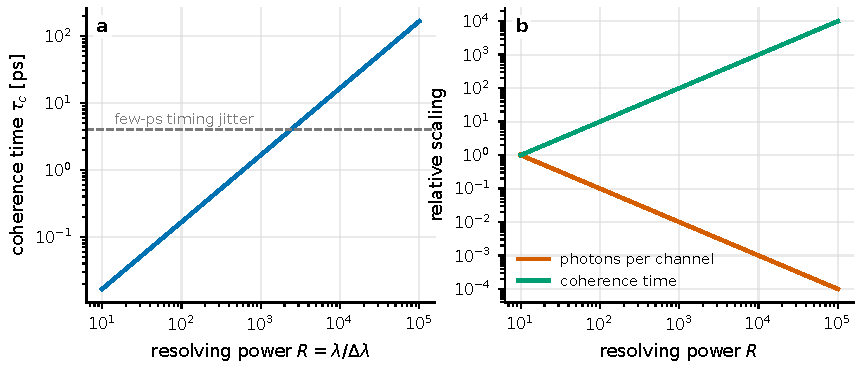
\includegraphics[width=0.92\linewidth]{figures/generated/chapter_06/ch06_spectral_resolution_coherence.pdf}
\caption{光谱分辨率与相干时间的数量级关系。左图固定 \(\lambda=500\,{\rm nm}\)，显示 \(\tau_c\simeq R\lambda/c\) 随分辨率线性增长；右图显示单通道光子率约随 \(1/R\) 降低，而相干时间随 \(R\) 增加。理想强度干涉的信噪比对光学带宽的依赖会部分抵消，但真实仪器还受滤光片形状、探测器响应、背景与电子带宽限制。}
\label{fig:e13-spectral-resolution-coherence}
\end{figure}

\section{本章要点}
\label{sec:e13-summary}

\begin{itemize}
  \item \textbf{光子变事件要过几道关卡。}量子效率 \(\eta\) 决定"多少光子变事件"（式 \eqref{eq:e13-detected-rate}）；PMT 大面积高增益、SPAD/SiPM 单光子皮秒计时但受面积、死时间、afterpulsing 限制，各有取舍。
  \item \textbf{抖动把相关峰卷宽、峰高稀释。}观测峰是真实峰与仪器响应的卷积（式 \eqref{eq:e13-response-convolution}）；独立高斯展宽按方差相加 \(\sigma_{\rm obs}^2=\sum\sigma_i^2\)（式 \eqref{eq:e13-jitter-budget}）。可见光 \(\tau_c\sim\)ps 远小于 ns 级响应，故峰宽几乎全由仪器决定，峰高被 \(\sim\sigma_{\rm sky}/\sigma_{\rm obs}\) 稀释——呼应第 \ref{chap:e08} 章。
  \item \textbf{死时间让记录率饱和，且分两型。}非麻痹型 \(r_{\rm rec}=r/(1+r\tau_d)\)（式 \eqref{eq:e13-nonparalyzable}）高通量饱和到 \(1/\tau_d\)；麻痹型 \(r_{\rm rec}=re^{-r\tau_d}\)（式 \eqref{eq:e13-paralyzable}）在 \(r\tau_d=1\) 达峰后回落。弱光下两者一致，强光下天差地别，必须实测判型。
  \item \textbf{afterpulsing 伪造短延迟假峰。}余脉冲率 \(R_{\rm ap}=\epsilon_{\rm ap}R_{\rm det}k_{\rm ap}(\tau)\)（式 \eqref{eq:e13-afterpulse}）落在关键的短延迟区。分束到两个独立探测器做互相关，能同时化解死时间与 afterpulsing。
  \item \textbf{时钟同步等价于对齐光程。}\(\Delta\ell=c\Delta t\)（式 \eqref{eq:e13-lightpath}）：100 ps \(\leftrightarrow\) 3 cm、1 ns \(\leftrightarrow\) 30 cm。GPS/White Rabbit 把两站对齐到几十皮秒；几何延迟 \(\Delta t_{\rm geo}=\mathbf B\cdot\hat{\mathbf s}/c\)（式 \eqref{eq:e13-geometric-delay}）最大（百米基线 \(\sim\)333 ns）且随地球自转漂移，须逐帧扣除。
  \item \textbf{事件表分三层、保原始信息。}原始层不可覆盖，标定层可迭代，相关产品层出成品；每个字段都对应一种"事后还想重做"的选择。可复现是最高准则。
  \item \textbf{谱分辨与相干时间此消彼长。}\(\tau_c\simeq R\lambda/c\)（式 \eqref{eq:e13-coherence-time}）：\(R\) 越大相干时间越长，但单通道光子率约降 \(1/R\)。选宽选窄取决于是测直径还是看速度结构。
\end{itemize}

\noindent\textbf{想一想。}(1) 若某 SPAD 的死时间曲线在高通量下先升后降，它更可能是哪一型？据此如何反推 \(\tau_d\)？(2) 把两站时钟对齐到 50 ps，等价于对齐多长的光程？这相对 100 m 基线的几何延迟是大是小？(3) 若把 \(R\) 从 100 提到 \(10^4\)，相干时间涨了多少倍，单通道光子率大约降到原来的几分之一？要保住总通量该怎么办？
